\chapter{Contexte général du projet}
\epigraph{Economists and agronomists are locked in debate about likely
future yields. Since the method of the economists is to predict
future outcomes from past performance, economists expect
success to continue. And since for the scientists future success
depends on discoveries they will have to make and do not now
know how to make, the scientists are doubtful. At its core, this is
a disagreement about the pace of technical change.}{Robert
Socolow}	
\subparagraph{}
Ce chapitre contextualise le projet dans son environment, en présentant en premier lieu l'organisme hôte de celui-ci – L'Office Chérifien des Phosphates – avant de motiver les raisons inhérentes à son implémentation pour finir sur la planification du déroulement de l'analyse, la conception et la réalisation du projet.
\cleardoublepage

\section{Présentation de l’OCP}
	\subsection{Historique}
	En 1920, alors que partout dans le monde, les compagnies minières fouillent fébrilement le
sous-sol à la recherche du phosphate, minerai aux précieuses vertus fertilisantes, l’Office
Chérifien des Phosphates (OCP S.A. depuis 2008) voit le jour.

En 1965, avec la mise en service du Maroc Chimie à Safi, le groupe devient également
exportateur de produits dérivés. En 1998, il franchit une nouvelle étape en lançant la fabrication
et l’exportation d’acide phosphorique purifié.

Parallèlement, de nombreux partenariats sont développés avec des opérateurs industriels du
secteur, au Maroc et à l’étranger.
	\subsection{Fiche signalétique}
	\begin{description}[align=left]
		\item [Nomination sociale :] Groupe Office Chérifien des Phosphates
		\item [Date de création :] 1920
		\item [Siège social :] 2-4, rue Al Abtal, Hay Erraha, 20200 Casablanca
		\item [Capital social :] 8287 M MAD (2013)
		\item [Effectif employé :] 23,000 (2013)
		\item [Site web :] www.ocpgroup.ma
	\end{description}
	\subsection{Quelques événements marquants de l’histoire du Groupe OCP}
	\begin{description}[align=left]
		\item [1920 :] Création, le 7 août, de l'office chérifien des Phosphates (OCP).
		\item [1959 :] Création de la société marocaine d'études spécialisées et industrielles (SMESI).
		\item [1965 :] Création de la société Maroc Chimie.
		\item [1974 :] Lancement des travaux pour la réalisation du centre minier de Benguérir, en mai.
		\item [1975 :] Création du Groupe OCP avec l'intégration des industries chimiques aux
		\item [1998 :] Le Groupe OCP obtient le Prix National de la Qualité.
		\item [2003 :] L'OCP est devenu le seul actionnaire de Phosboucraâ.
		\item [2008 :] La société anonyme OCP SA est née le 22 janvier - Démarrage de Pakistan Maroc
		\item [2009 :] Démarrage de Bunge Maroc Phosphore à Jorf Lasfar (BMP).
		\item [2010 :] Création de JESA, joint-venture sous forme de partenariat en ingénierie
		\item [2012 :] Creation de la JV BSFT (Black Sea Fertilizer Trading Company)
		\item [2013 :] Signature d’une joint-venture avec Dupont
		\item [2014 :] Inauguration du SLURRY PIPELINE entre Khouribga et Jorf Lasfar
	\end{description}
	
	\subsection{Filiales et Partenariats}
	L'OCP se structure en quatre filières chacune se focalisant sur un segment du groupe OCP et ayant co-créé plusieurs coentreprises dont la figure \ref{fig:mesh1} fait la liste : 
	\begin{figure}[h]
    		\centering
    		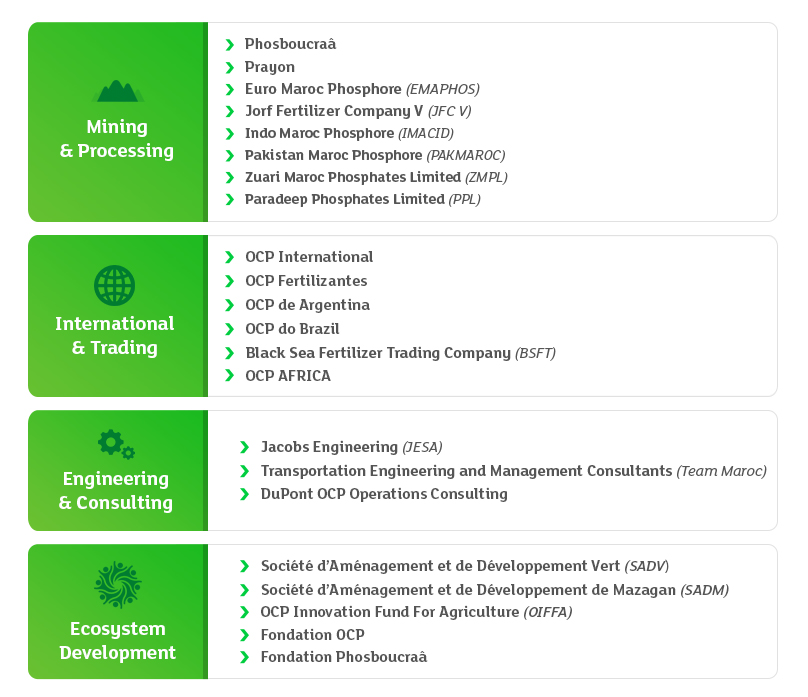
\includegraphics[scale=0.62]{Companies-ocp}
    		\caption{Filiales et Coentreprises de l’OCP\cite{ocp-fil}}
    		\label{fig:mesh1}
	\end{figure}
	
	
\section{Présentation du projet}
	\subsection{Cadre général du projet}
	
	\subsection{Motivation et Problématique}
	\subsubsection{Motivation}
	Parce que la demande d'engrais dépend d'une variété de facteurs agro-économiques, celle-ci n’est pas stable, ni est-elle sujette à des prédictions exactes. Le choix des méthodes de prévision est donc particulièrement important, tant pour la gestion efficiente des compagnies productrices des engrais que pour la formulation de politiques appropriées par les gouvernements.
	La prévision efficace de la demande peut permettre aux exportateurs de tirer pleinement parti des fluctuations des cours mondiaux du marché. Le stockage requis, le transport, les ressources humaines à mobiliser, les arrangements financiers de crédits et de devises étrangères sont tributaires de la demande.
	\paragraph{}
	Considérant que les engrais produits mais non vendus peuvent être conservés pendant un an avant de trouver un acheteur et qu'une durée de stockage d'une année peut causer des partes en quantité et en qualité conséquentes, l'importance de la prévision de la demande peut être facilement appréciée. Si la demande réelle est plus grande que prévue, ce ci conduit à des pénuries, une production agricole inférieure et, souvent, à des implications politiques pour les pays importateurs.
	\paragraph*{}
	Tous les plans des entreprises fabriquant ou commercialisant des engrais devraient être dérivés directement ou indirectement de la prévision de la demande. A partir d'une prévision internationale de la demande, les ventes attendues d'une entreprise peuvent être estimées en évaluant sa part de marché dans chaque région du pays.
	\paragraph{}
	La prévision des ventes servira de consigne à l’égard du département de production quant à quoi, quand et combien produire. Le département financier de l'OCP, lui, est ainsi en mesure de préparer, sur la base des prévisions de ventes, un plan d'entrées et sorties de fonds, évaluer l'écart entre les fonds de roulement et d'organiser le soutien nécessaire de la banque. Le département marketing est guidé par la prévision dans le déploiement du personnel de vente, alors que le logistique sera éclairé quant à l’organisation du stockage à des endroits appropriés, les contrats de transport de marchandises pour faire face au volume prévu de l'entreprise.
	\subsubsection{Problématique}
Au fil des années, la direction commerciale-marketing où nous avons effectué notre stage de fin d'études, a itérativement modernisé ses outils de traitement d'information. Dernière contribution en date de L'ENSIAS\footnote{Ecole Nationale Supérieure d'Informatique et d'Analyse des Systèmes - Grande Ecole d'Ingénieurs, Maroc} à cet essort informationnel, a consisté en la mise en place d'une solution adéquate basée sur les concepts et technologies du BI\footnote{Business Intelligence} ayant permis l'automatisation de la reception, de la normatlisation et l'exploitation de tableau de bord post-analyse des données recuillies\cite{NACER}. La plateforme ainsi réalisée par notre prédecesseur est ainsi un socle pour aider les décionnaires CM\footnote{Commercial-Marketing} à mieux appréhender les évolution et historiques des marchés mondiaux.\paragraph{}Ces données proviennent des organismes indépendants spécialisés dans l'analyse de marché. Hebdomadairement, la direction commerciale reçoit plus de 100 publications de ces organismes qui contiennent des guides de prix, des évaluations ou même des prévisions concernant le marché de phosphates, ses dérivées et les matières premières.\paragraph{}Nous proposons d'emmener les perspectives informationelles du département CM au-delà du reporting \footnote{Tableaux de bord et rapports Business Intelligence} continu vers des mécanismes décisionnels et prévisionnels mettant en œuvre les techniques à l'état de l'art de fouilles de données (cf def data mining) . Nous souhaitons ainsi 'miner' des relations interessantes régissant le marché international des phosphates qui ne sauraient être mises en relief par les techniques de la BI à savoir la segmentation en faits, dimensions et mesures. Notre problématique s'articule ainsi:\subparagraph*{}\textbf{Quelles mécanismes prévisionnels peuvent être établis à la suite d'une recherche de structure précedemment inconnue dans le marché international des phosphates ?}\subparagraph*{}Répondre d'une manière exhaustive à cette question constituerait un atout clé en faveur d'une meilleure compétitivité de l'OCP et nous nous proposons d'explorer divers piste dont le présent rapport témoigne. 
\section{Planification du projet}
	\subsection{Les étapes CRISP-DM d'un projet Data Mining}
	\subsection{Le planning du projet}